
Ici sont rassemblés les notes, idées et résultats obtenus jusqu'à présent.

\subsection{Rappel personnel} % (fold)
\label{sub:rappel_personnel}

Rappel de cours : les fonctions d'activation comme tanh ou sigmoïde peuvent 
saturer. En général un pas d'apprentissage de l'ordre de 1 est salutaire pour 
pouvoir sortir de l'état saturé. De plus le gradient est borné. Il n'y a donc 
pas de risque de mise à jour trop violente des poids.

Cependant ReLU ne suit pas cette règle. Le gradient n'étant pas borné pour 
cette activation il est recommandé de commencer avec un pas d'apprentissage
faible (de l'ordre de 0.01) afin d'éviter les mises à jour trop violente.

Enfin un pas trop petit pour tanh ou sigmoïde peut être très préjudiciable.
Le gradient serait alors trop petit donc très sensible au bruit.
La descente de gradient reviendrait à demander à une fourmi de trouver la 
vallée dans une route rocailleuse. Elle serait facilement bloquée dans un
minimum local.

Passer de ReLU à tanh ou sigmoïde requiert donc systématiquement d'adapter
le pas d'apprentissage.

% subsection rappel_personnel (end)
\subsection{Reverse gradient layer astuces} % (fold)
\label{sub:reverse_gradient_layer_astuce}

RGL : $\lambda_D = -1 \iff \cancel{\text{RGL}}$

Choisir $\lambda_D = -1$ est équivalent à ne pas avoir de RGL, le gradient se 
retrouve inchangé ($grad \gets -1\times-1\times grad $).

RGL : $\lambda_D = 0 \iff \cancel{\text{Adaptation}}$

Choisir $\lambda_D = 0$ est équivalent à ne pas avoir d'adaptation, le 
gradient se retrouve bloqué par le RGL ($grad \gets -1\times0\times grad $).

En théorie un DANN parfait est un DANN dont la partie classification du
domaine se comporte comme le hasard, la distribution rendant parfaitement
indissociable l'origine des exemples.

Dans la pratique des DANN répondant systèmatiquement le même domaine n'ont 
pas toujours montrés des comportements pathologiques. 
C'est donc au cas par cas ?
En tout cas le visionnage de la matrice de confusion de la sortie "Domaine" du
DANN peut servir et ne coûte pas chère.

% subsection reverse_gradient_layer_astuces (end)
\subsection{Moons} % (fold)
\label{sub:moons}
Commençons pas l'application sur des données artificielles simples et 
facilement interprétables.

L'exemple des 2 lunes imbriquées est un problème non linéaire simple. Un
réseaux de neurone à 1 couche caché de 3 neurones permet de le résoudre
à la perfection.

\begin{figure}[htbp]
\centering
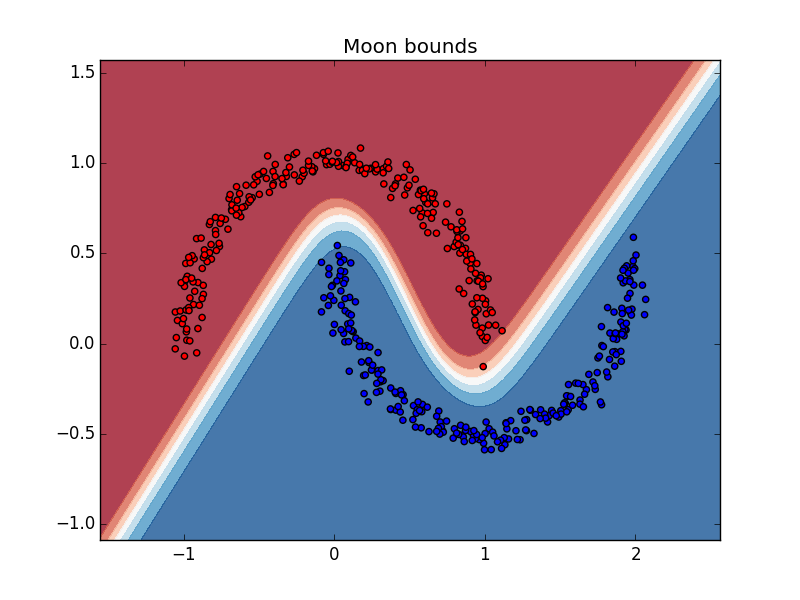
\includegraphics[width=\columnwidth]{fig/moon-bound-0.png}
\caption{Moon classique}
\end{figure}

On peut simuler un problème d'adaptation en appliquant une petite
transformation sur ces données.
Après une rotation de 35 degrés des données le réseau de base perd une bonne
partie de ses performances. On définit donc le domaine Source et Cible
comme étant respectivement les données originelles et les données après
rotation.

L'utilisation d'un \emph{DANN} permet de réduire en partie la perte de 
performance en adaptant le réseau à ces nouvelles données (cf figure \ref{fig:moonrot}.

\begin{figure}[htbp]
\centering
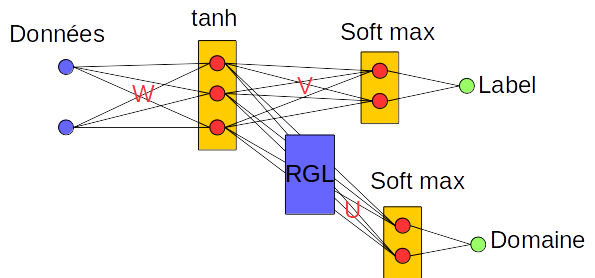
\includegraphics[width=\columnwidth]{fig/DANN-simple.png}
\caption{Structure minimale d'un DANN. (utilisé pour Moon)}
\end{figure}

\begin{figure*}[htbp]
\centering
\subfigure[Sans le DANN les performances sont diminuées.]
	{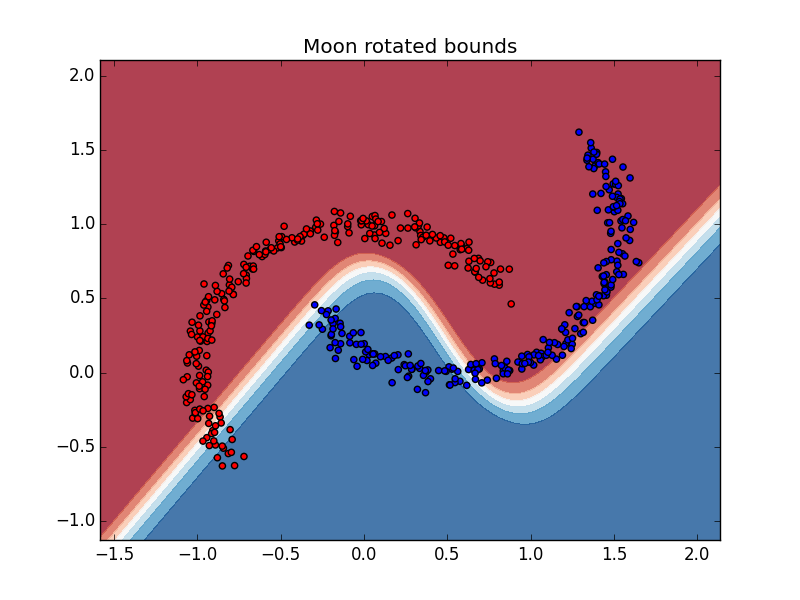
\includegraphics[width=\columnwidth]{fig/moon-rot-bound-0.png}}
\hfill
\subfigure[En appliquant un DANN on peut partiellement corriger ce problème
($\lambda_D=0.7$)]
	{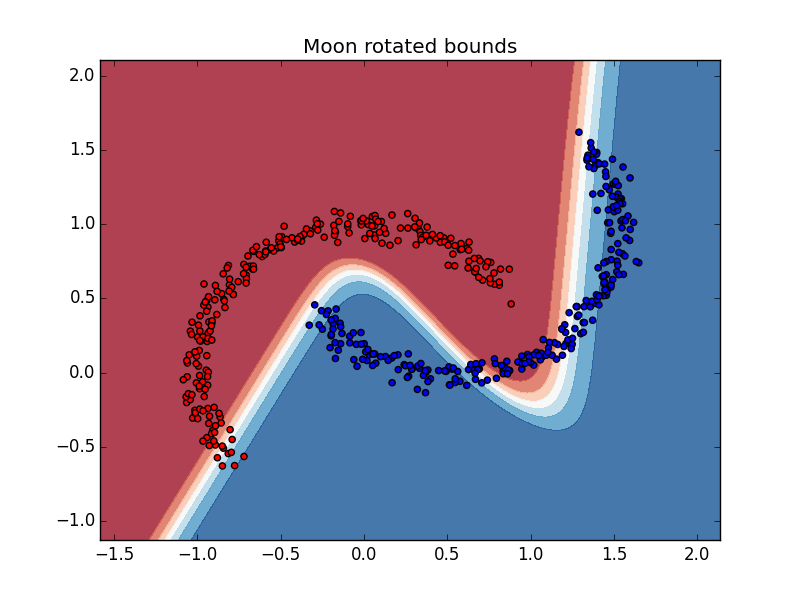
\includegraphics[width=\columnwidth]{fig/moon-rot-bound-1.png}}
\caption{Moon après une rotation de 35 degrés.}
\label{fig:moonrot}

\centering
\subfigure[Avant l'utilisation du DANN.]
	{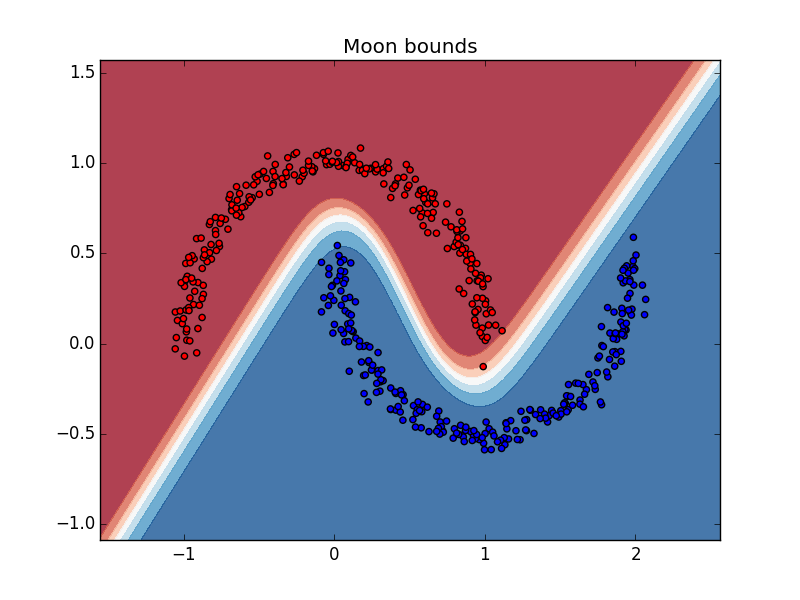
\includegraphics[width=\columnwidth]{fig/moon-bound-0.png}}
\hfill
\subfigure[Le DANN ne fait pas perdre de performances sur ces données.]
	{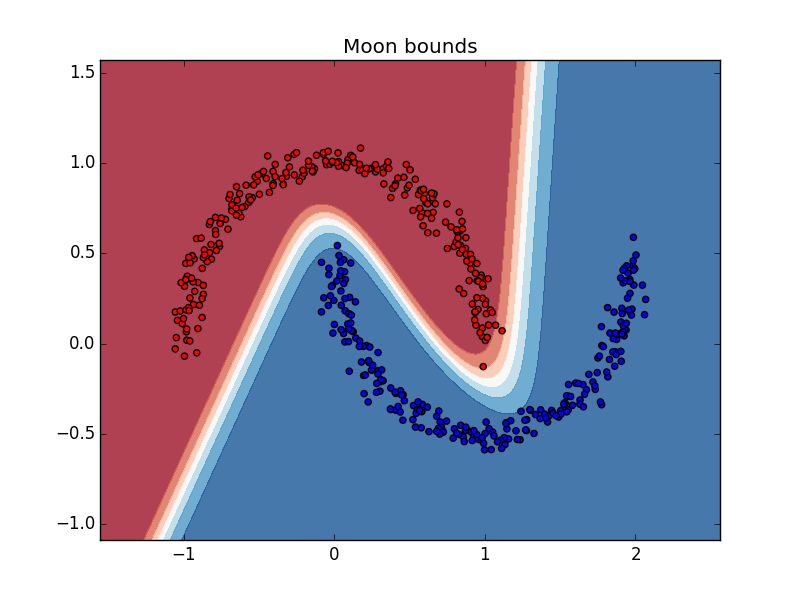
\includegraphics[width=\columnwidth]{fig/moon-bound-1.png}}
\caption{Moon (donnée originale).}
\end{figure*}

Une autre transformation consiste à appliquer une matrice à dominance
diagonale aux données:

$ x \gets A.x $ où $A$ est une matrice à dominance diagonale $(2\times2)$
générée aléatoirement.

On obtient des résultats similaire (cf figure \ref{fig:moonA}).

\begin{figure*}[htbp]
\centering
\subfigure[Sans le DANN.]
	{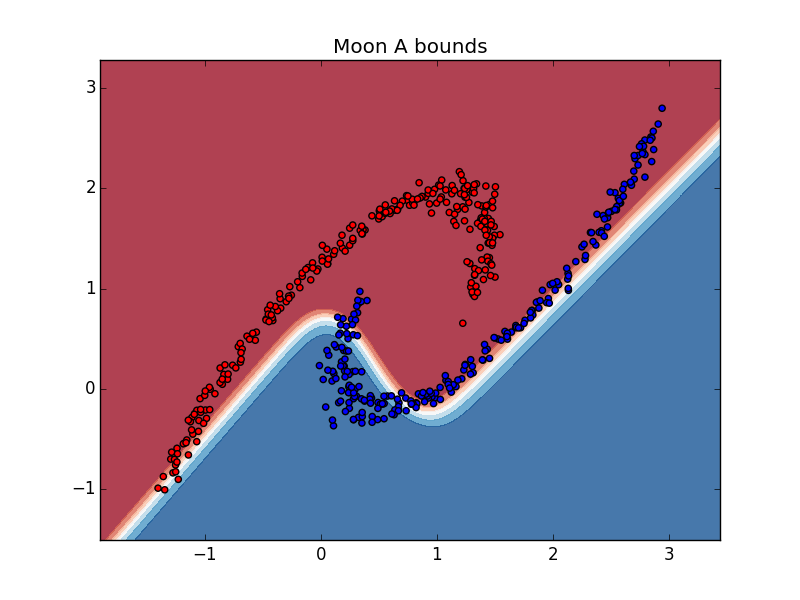
\includegraphics[width=\columnwidth]{fig/moon-A-bound-0.png}}
\hfill
\subfigure[En appliquant un DANN ($\lambda_D=0.7$)]
	{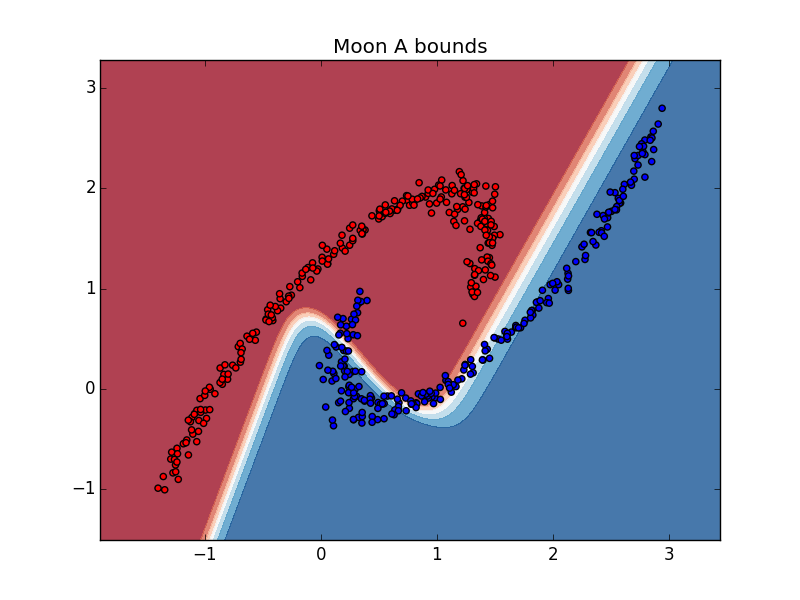
\includegraphics[width=\columnwidth]{fig/moon-A-bound-1.png}}
\caption{Moon après application de $A$.}
\label{fig:moonA}
\end{figure*}


% \FloatBarrier
% subsection moons (end)

\subsection{MNIST} % (fold)
\label{sub:mnist}

Étudions maintenant un problème réel à plus grande dimension.
MNIST est le jeu de données le plus classique. Commençons par utiliser la 
transformation en passant par une matrice à dominance diagonale.

$ x \gets A.x $ où $A$ est une matrice à dominance diagonale $(748\times748)$
générée aléatoirement.

Les données ne sont pas grandement modifiées par cette transformation. 
Les changement sont pas visible à l'oeil nu (figure \ref{fig:MNIST-A-sample})

\begin{figure}[htbp]
\centering
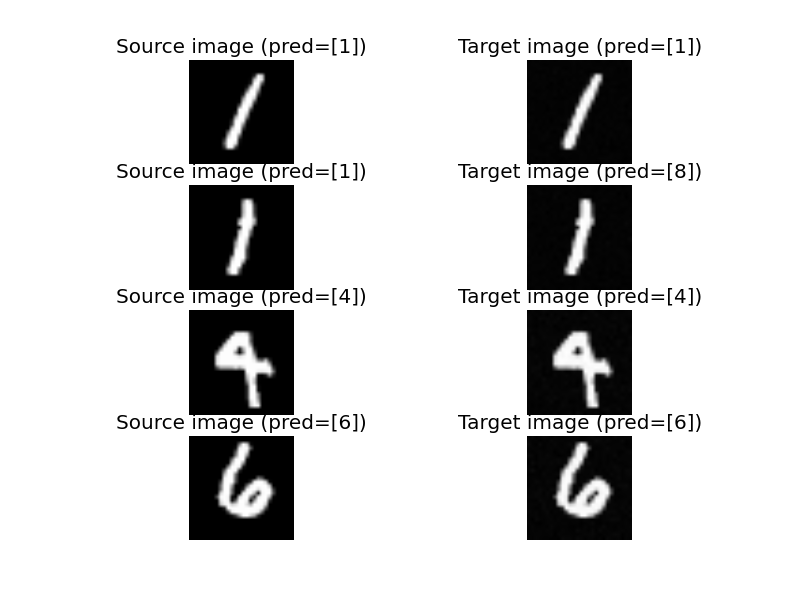
\includegraphics[width=\columnwidth]{fig/MNIST-A-sample.png}
\caption{Examples sur MNIST et MNIST après application d'une matrice à dominance diagonale aléatoire.}
\label{fig:MNIST-A-sample}
\end{figure}

La structure est la même que pour les données \emph{Moons classiques}. 
Un réseaux à une seule couche caché. Cependant la couche cachée compte
maintenant 50 neurones.

Comme on peut le remarquer figure \ref{fig:MNISTA}, le réseaux sans la partie
adaptation fait peu à peu chuter la précision sur les données transformées.
L'utilisation du DANN permet de limiter cette perte de performance.

\begin{figure*}[htbp]
\centering
\subfigure[Sans le DANN.]
	{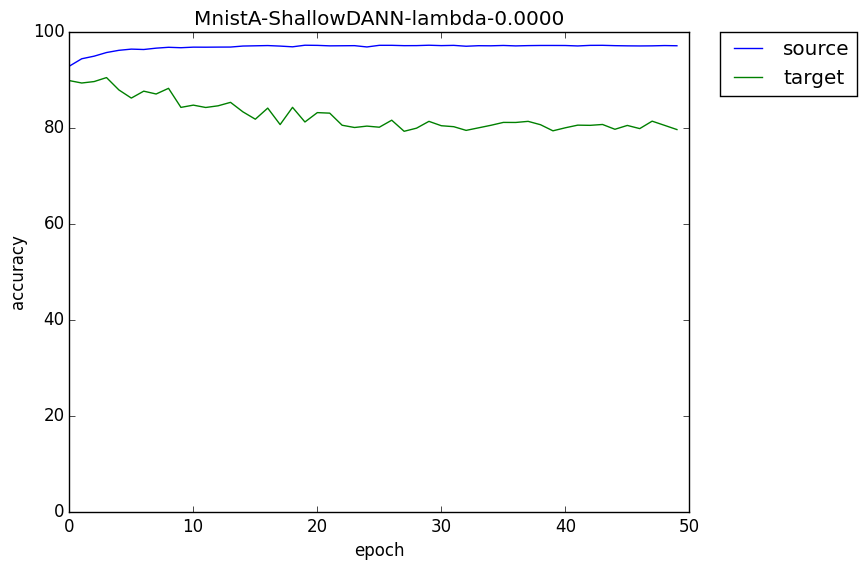
\includegraphics[width=\columnwidth]{fig/MnistA-ShallowDANN-lambda-0.png}}
\hfill
\subfigure[En appliquant un DANN ($\lambda_D=0.01$)]
	{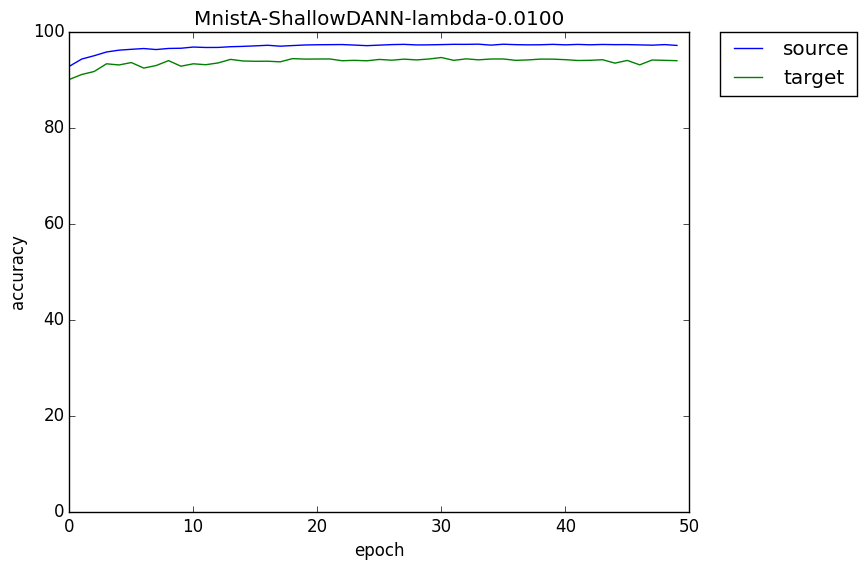
\includegraphics[width=\columnwidth]{fig/MnistA-ShallowDANN-lambda-0,0100.png}}
\caption{Évolution de la précision sur le set de validation sur MNIST et MNIST
	après application d'une matrice à dominance diagonale aléatoire.}
\label{fig:MNISTA}
\end{figure*}

Une autre transformation consiste à appliquer une permutation des pixels.
Dans le cas de MNIST on peut par exemple renverser l'image selon un axe 
(figure \ref{fig:MNIST-Mirror-sample}).

\begin{figure}[htbp]
\centering
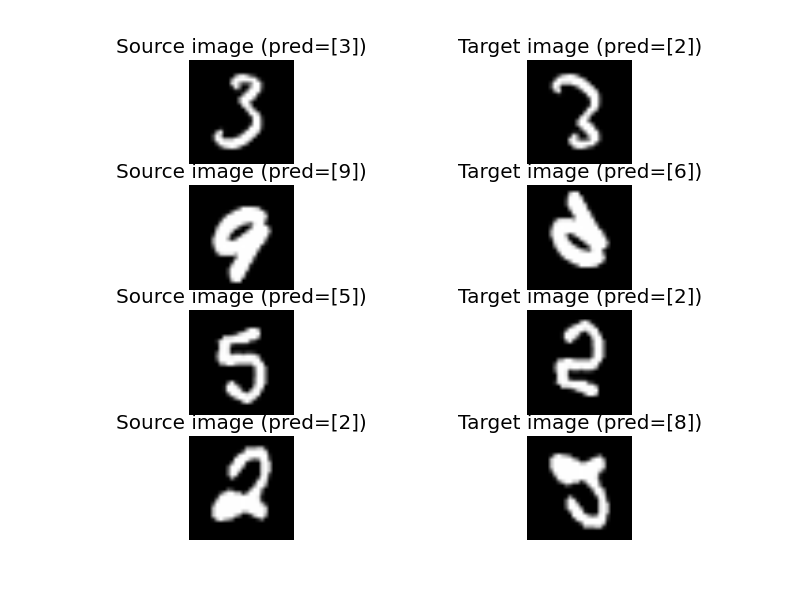
\includegraphics[width=\columnwidth]{fig/MNIST-Mirror-sample.png}
\caption{Examples sur MNIST et MNIST après renversement.}
\label{fig:MNIST-Mirror-sample}
\end{figure}

Cependant cette fois ci le DANN ne semble pas capable de corriger le modèle.
Après avoir essayer diverses configurations et hyper-paramètre j'ai conclu que
la transformation était trop importante pour réussir l'adaptation.

Bien entendu un réseau de neurone avec une couche de convolution règle le 
problème sans même avoir besoin d'adaptation. Mais pour un réseau constitué 
uniquement de couches denses, je n'ai pas obenu de représentation commune 
par entraînement d'un DANN.

Cette fois ci l'architecture utilisée pour la représentation est un peu plus 
complexe : 3 couches denses avec dropout à 50\% et ReLU construite avec 
respectivement 392, 196 et 98 neurones.

Les résultats sont indiqués sous la forme de matrice de confusion figure
\ref{fig:MNIST-Mirror-CM}.

\begin{figure*}[htbp]
\centering
\subfigure[Sans le DANN. $\lambda_D=0$)]
	{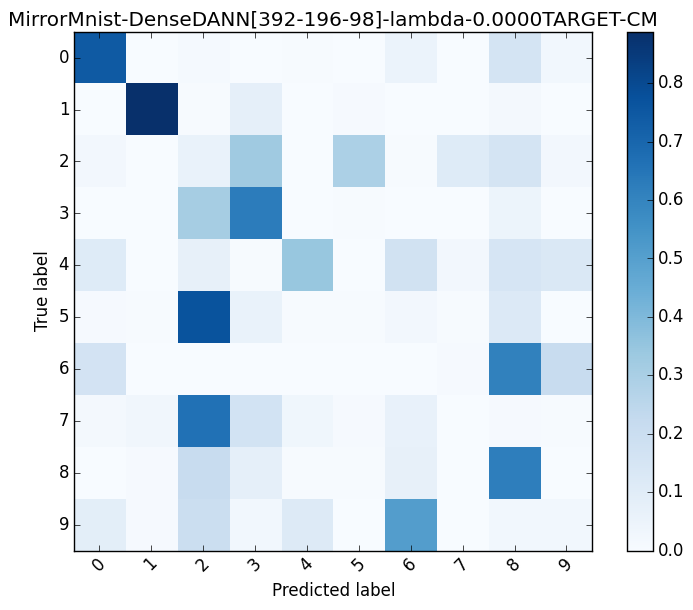
\includegraphics[width=\columnwidth]{fig/MirrorMnist-DenseDANN[392-196-98]-lambda-0,0000TARGET-CM.png}}
\hfill
\subfigure[En appliquant un DANN ($\lambda_D=0.01$)]
	{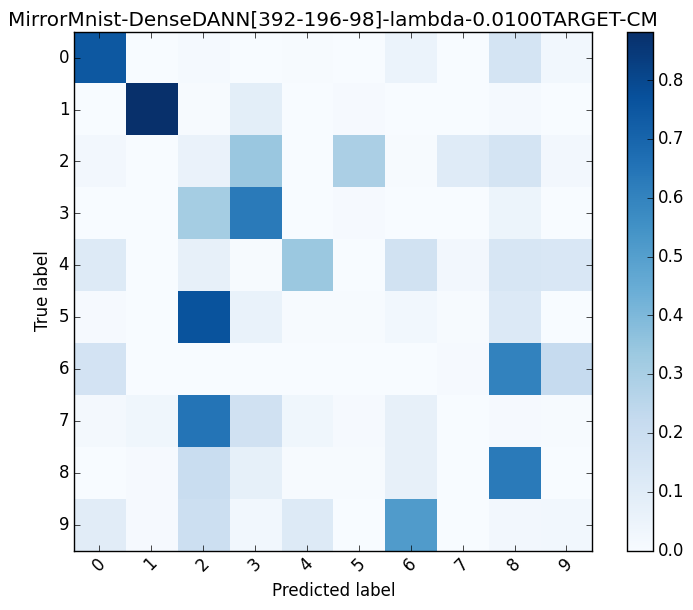
\includegraphics[width=\columnwidth]{fig/MirrorMnist-DenseDANN[392-196-98]-lambda-0,0100TARGET-CM.png}}
\subfigure[Sans le DANN. $\lambda_D=0.1$)]
	{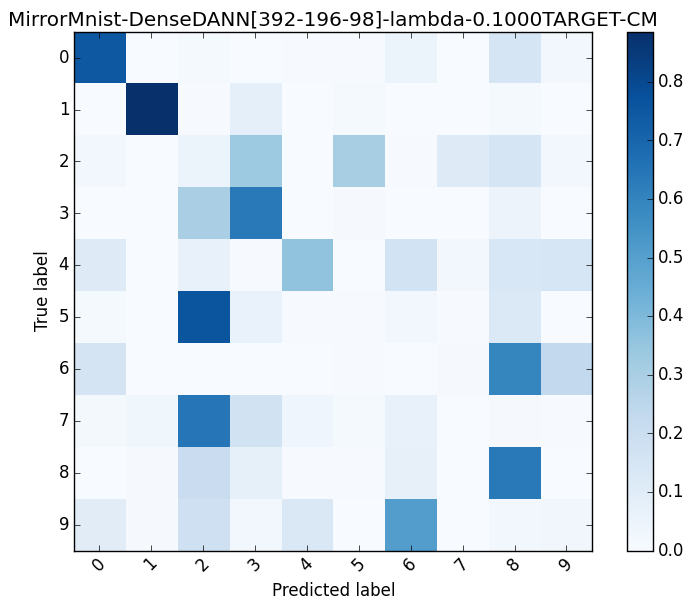
\includegraphics[width=\columnwidth]{fig/MirrorMnist-DenseDANN[392-196-98]-lambda-0,1000TARGET-CM.png}}
\hfill
\subfigure[En appliquant un DANN ($\lambda_D=1.0$)]
	{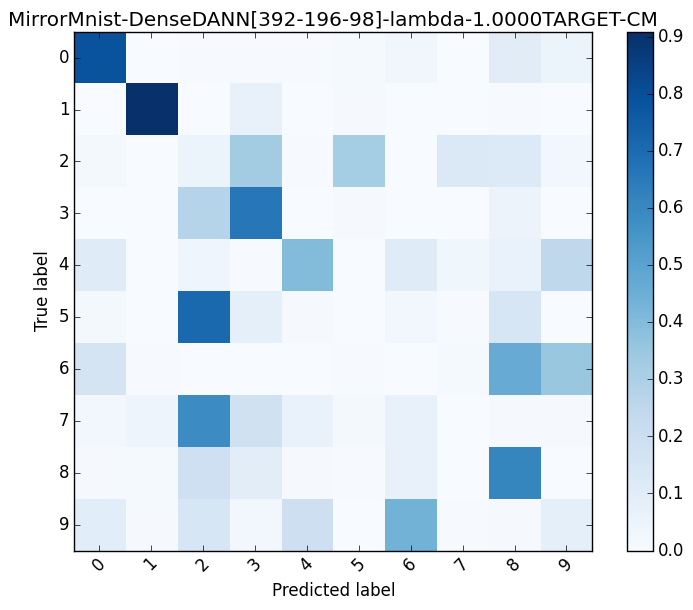
\includegraphics[width=\columnwidth]{fig/MirrorMnist-DenseDANN[392-196-98]-lambda-1,0000TARGET-CM.png}}
\caption{Évolution de la précision sur le set de validation sur MNIST et MNIST
	après application d'une matrice à dominance diagonale aléatoire.}
\label{fig:MNIST-Mirror-CM}
\end{figure*}

% subsection mnist (end)
